\testfile{pgfplotstest.axislines.3d.tex}
{
	\pgfplotsset{
		samples=5,
		domain=-4:4,
		xtick=data,
		ytick=data,
	%	ztick=data,
	}

	\testsection{Boxed}
	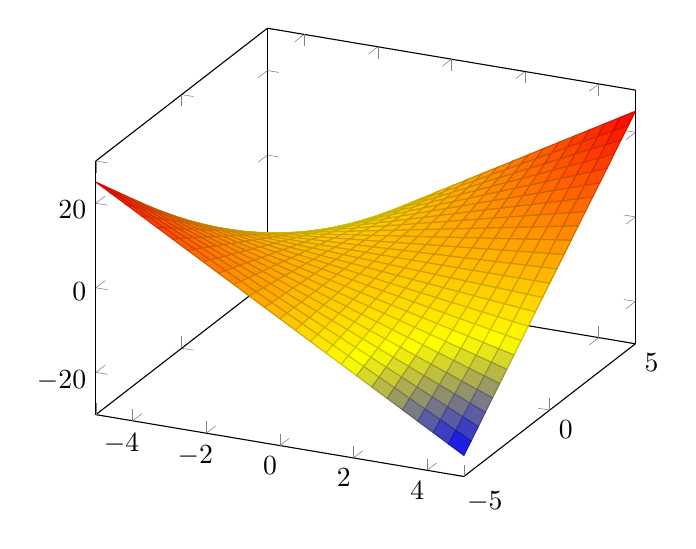
\begin{tikzpicture}
		\begin{axis}[]
			\addplot3[surf] {x*y};
		\end{axis}
	\end{tikzpicture}

	\testsection{axis lines=left}
	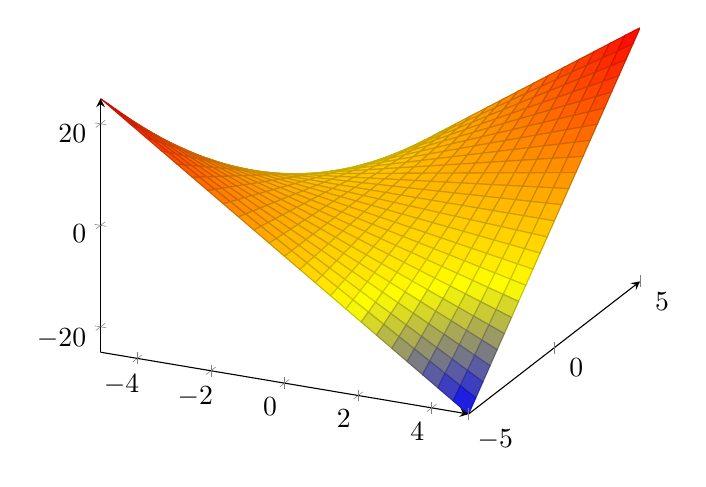
\begin{tikzpicture}
		\begin{axis}[
			axis on top,
			axis lines=left,
		]
			\addplot3[surf] {x*y};
		\end{axis}
	\end{tikzpicture}

	\testsection{axis lines=right}
	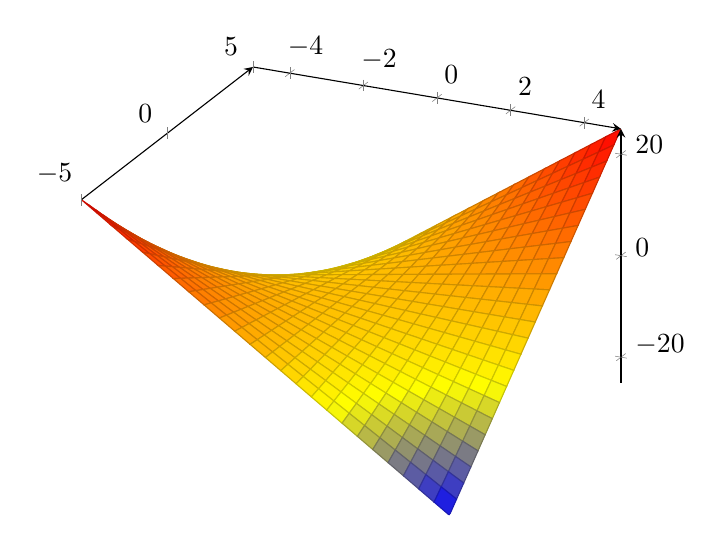
\begin{tikzpicture}
		\begin{axis}[
			axis on top,
			axis lines=right,
		]
			\addplot3[surf] {x*y};
		\end{axis}
	\end{tikzpicture}

	\testsection{axis lines=middle,axis on top}
	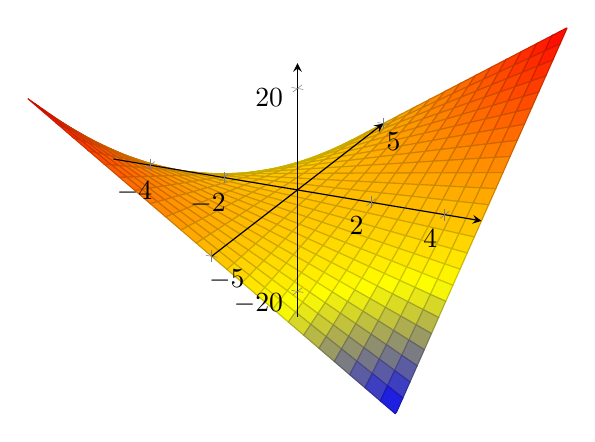
\begin{tikzpicture}
		\begin{axis}[
			axis on top,
			axis lines=middle,
		]
			\addplot3[surf] {x*y};
		\end{axis}
	\end{tikzpicture}

	\testsection{Only  axis x line=middle}
	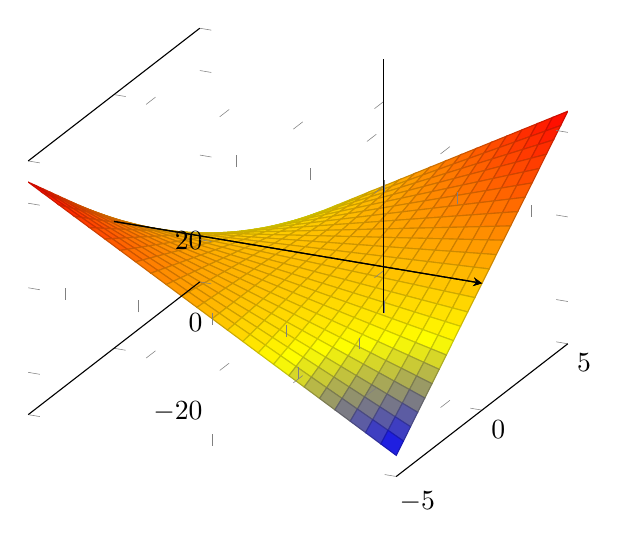
\begin{tikzpicture}
		\begin{axis}[axis on top,
			axis x line=middle,
		]
			\addplot3[surf] {x*y};
		\end{axis}
	\end{tikzpicture}


	\testsection{3d box=complete}
	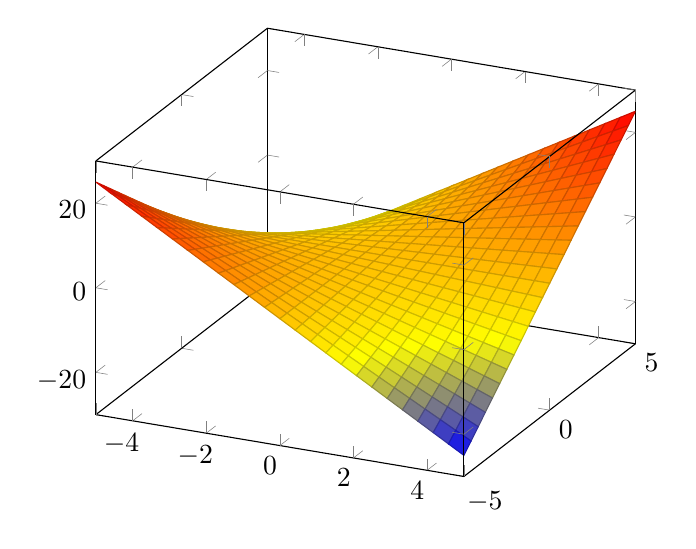
\begin{tikzpicture}
		\begin{axis}[
			3d box=complete,
		]
			\addplot3[surf] {x*y};
		\end{axis}
	\end{tikzpicture}
	
	\testsubsection{grid lines}
	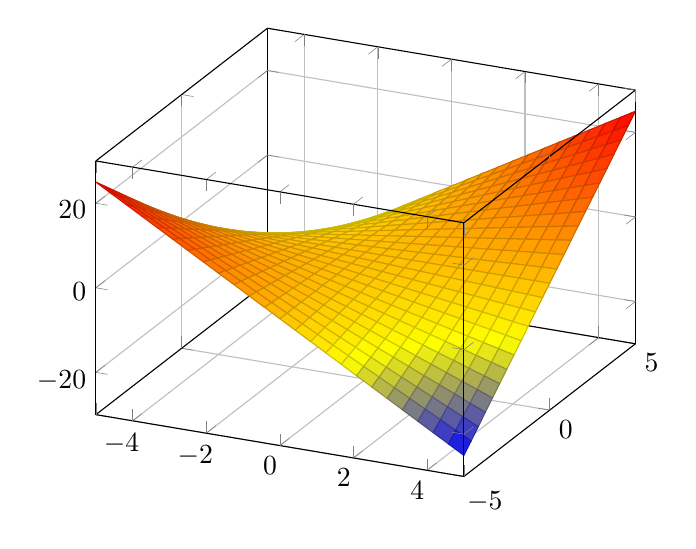
\begin{tikzpicture}
		\begin{axis}[
			grid=major,
			3d box=complete,
		]
			\addplot3[surf] {x*y};
		\end{axis}
	\end{tikzpicture}

	\testsubsection{grid lines und completeSTAR}
	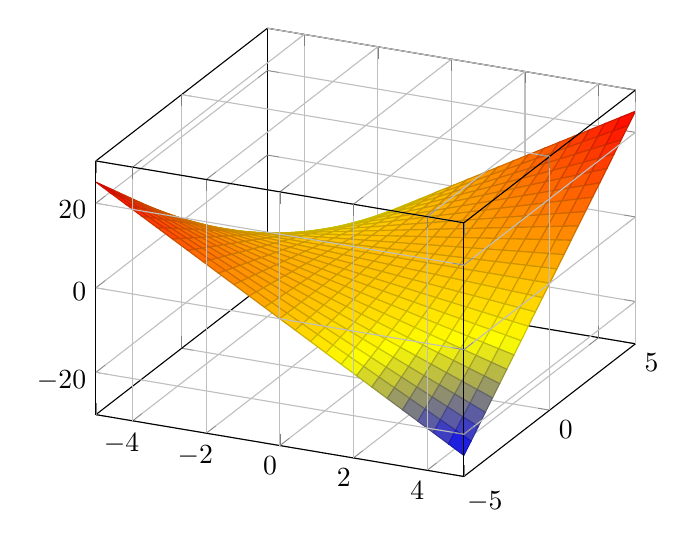
\begin{tikzpicture}
		\begin{axis}[
			grid=major,
			3d box=complete*,
		]
			\addplot3[surf] {x*y};
		\end{axis}
	\end{tikzpicture}

	\testsubsection{grid lines und completeSTAR und styles}
	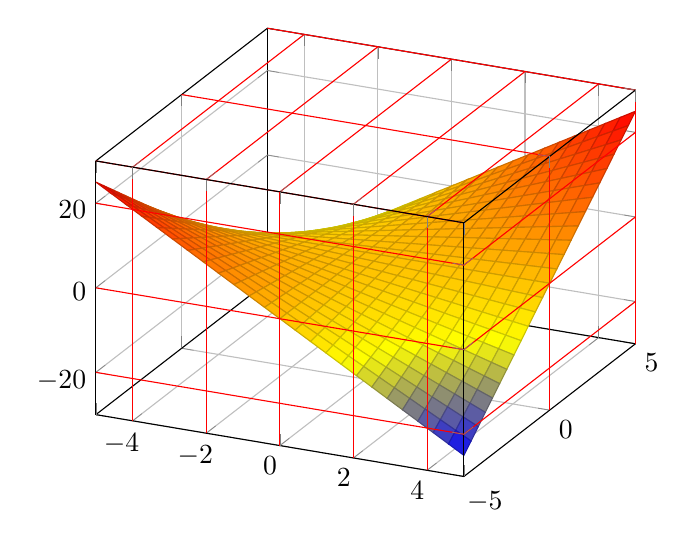
\begin{tikzpicture}
		\begin{axis}[
			grid=major,
			3d box=complete*,
			3d box foreground style={grid style={red}},
		]
			\addplot3[surf] {x*y};
		\end{axis}
	\end{tikzpicture}
}
